% Options for packages loaded elsewhere
\PassOptionsToPackage{unicode}{hyperref}
\PassOptionsToPackage{hyphens}{url}
%
\documentclass[
  english,
  man]{apa6}
\title{EDLD 653 Final Project}
\author{Anisha Babu, Ian Shryock, Dillon Welindt, Futing Zou, Diana DeWald\textsuperscript{1}}
\date{}

\usepackage{amsmath,amssymb}
\usepackage{lmodern}
\usepackage{iftex}
\ifPDFTeX
  \usepackage[T1]{fontenc}
  \usepackage[utf8]{inputenc}
  \usepackage{textcomp} % provide euro and other symbols
\else % if luatex or xetex
  \usepackage{unicode-math}
  \defaultfontfeatures{Scale=MatchLowercase}
  \defaultfontfeatures[\rmfamily]{Ligatures=TeX,Scale=1}
\fi
% Use upquote if available, for straight quotes in verbatim environments
\IfFileExists{upquote.sty}{\usepackage{upquote}}{}
\IfFileExists{microtype.sty}{% use microtype if available
  \usepackage[]{microtype}
  \UseMicrotypeSet[protrusion]{basicmath} % disable protrusion for tt fonts
}{}
\makeatletter
\@ifundefined{KOMAClassName}{% if non-KOMA class
  \IfFileExists{parskip.sty}{%
    \usepackage{parskip}
  }{% else
    \setlength{\parindent}{0pt}
    \setlength{\parskip}{6pt plus 2pt minus 1pt}}
}{% if KOMA class
  \KOMAoptions{parskip=half}}
\makeatother
\usepackage{xcolor}
\IfFileExists{xurl.sty}{\usepackage{xurl}}{} % add URL line breaks if available
\IfFileExists{bookmark.sty}{\usepackage{bookmark}}{\usepackage{hyperref}}
\hypersetup{
  pdftitle={EDLD 653 Final Project},
  pdfauthor={Anisha Babu, Ian Shryock, Dillon Welindt, Futing Zou, Diana DeWald1},
  pdflang={en-EN},
  pdfkeywords={Personality traits, SAPA-Project Dataverse, Functional Programming},
  hidelinks,
  pdfcreator={LaTeX via pandoc}}
\urlstyle{same} % disable monospaced font for URLs
\usepackage{graphicx}
\makeatletter
\def\maxwidth{\ifdim\Gin@nat@width>\linewidth\linewidth\else\Gin@nat@width\fi}
\def\maxheight{\ifdim\Gin@nat@height>\textheight\textheight\else\Gin@nat@height\fi}
\makeatother
% Scale images if necessary, so that they will not overflow the page
% margins by default, and it is still possible to overwrite the defaults
% using explicit options in \includegraphics[width, height, ...]{}
\setkeys{Gin}{width=\maxwidth,height=\maxheight,keepaspectratio}
% Set default figure placement to htbp
\makeatletter
\def\fps@figure{htbp}
\makeatother
\setlength{\emergencystretch}{3em} % prevent overfull lines
\providecommand{\tightlist}{%
  \setlength{\itemsep}{0pt}\setlength{\parskip}{0pt}}
\setcounter{secnumdepth}{-\maxdimen} % remove section numbering
% Make \paragraph and \subparagraph free-standing
\ifx\paragraph\undefined\else
  \let\oldparagraph\paragraph
  \renewcommand{\paragraph}[1]{\oldparagraph{#1}\mbox{}}
\fi
\ifx\subparagraph\undefined\else
  \let\oldsubparagraph\subparagraph
  \renewcommand{\subparagraph}[1]{\oldsubparagraph{#1}\mbox{}}
\fi
\newlength{\cslhangindent}
\setlength{\cslhangindent}{1.5em}
\newlength{\csllabelwidth}
\setlength{\csllabelwidth}{3em}
\newlength{\cslentryspacingunit} % times entry-spacing
\setlength{\cslentryspacingunit}{\parskip}
\newenvironment{CSLReferences}[2] % #1 hanging-ident, #2 entry spacing
 {% don't indent paragraphs
  \setlength{\parindent}{0pt}
  % turn on hanging indent if param 1 is 1
  \ifodd #1
  \let\oldpar\par
  \def\par{\hangindent=\cslhangindent\oldpar}
  \fi
  % set entry spacing
  \setlength{\parskip}{#2\cslentryspacingunit}
 }%
 {}
\usepackage{calc}
\newcommand{\CSLBlock}[1]{#1\hfill\break}
\newcommand{\CSLLeftMargin}[1]{\parbox[t]{\csllabelwidth}{#1}}
\newcommand{\CSLRightInline}[1]{\parbox[t]{\linewidth - \csllabelwidth}{#1}\break}
\newcommand{\CSLIndent}[1]{\hspace{\cslhangindent}#1}
% Manuscript styling
\usepackage{upgreek}
\captionsetup{font=singlespacing,justification=justified}

% Table formatting
\usepackage{longtable}
\usepackage{lscape}
% \usepackage[counterclockwise]{rotating}   % Landscape page setup for large tables
\usepackage{multirow}		% Table styling
\usepackage{tabularx}		% Control Column width
\usepackage[flushleft]{threeparttable}	% Allows for three part tables with a specified notes section
\usepackage{threeparttablex}            % Lets threeparttable work with longtable

% Create new environments so endfloat can handle them
% \newenvironment{ltable}
%   {\begin{landscape}\centering\begin{threeparttable}}
%   {\end{threeparttable}\end{landscape}}
\newenvironment{lltable}{\begin{landscape}\centering\begin{ThreePartTable}}{\end{ThreePartTable}\end{landscape}}

% Enables adjusting longtable caption width to table width
% Solution found at http://golatex.de/longtable-mit-caption-so-breit-wie-die-tabelle-t15767.html
\makeatletter
\newcommand\LastLTentrywidth{1em}
\newlength\longtablewidth
\setlength{\longtablewidth}{1in}
\newcommand{\getlongtablewidth}{\begingroup \ifcsname LT@\roman{LT@tables}\endcsname \global\longtablewidth=0pt \renewcommand{\LT@entry}[2]{\global\advance\longtablewidth by ##2\relax\gdef\LastLTentrywidth{##2}}\@nameuse{LT@\roman{LT@tables}} \fi \endgroup}

% \setlength{\parindent}{0.5in}
% \setlength{\parskip}{0pt plus 0pt minus 0pt}

% \usepackage{etoolbox}
\makeatletter
\patchcmd{\HyOrg@maketitle}
  {\section{\normalfont\normalsize\abstractname}}
  {\section*{\normalfont\normalsize\abstractname}}
  {}{\typeout{Failed to patch abstract.}}
\patchcmd{\HyOrg@maketitle}
  {\section{\protect\normalfont{\@title}}}
  {\section*{\protect\normalfont{\@title}}}
  {}{\typeout{Failed to patch title.}}
\makeatother
\shorttitle{The Personality Structures of the 50 States}
\keywords{Personality traits, SAPA-Project Dataverse, Functional Programming\newline\indent Word count: 1106}
\DeclareDelayedFloatFlavor{ThreePartTable}{table}
\DeclareDelayedFloatFlavor{lltable}{table}
\DeclareDelayedFloatFlavor*{longtable}{table}
\makeatletter
\renewcommand{\efloat@iwrite}[1]{\immediate\expandafter\protected@write\csname efloat@post#1\endcsname{}}
\makeatother
\usepackage{lineno}

\linenumbers
\usepackage{csquotes}
\ifXeTeX
  % Load polyglossia as late as possible: uses bidi with RTL langages (e.g. Hebrew, Arabic)
  \usepackage{polyglossia}
  \setmainlanguage[]{english}
\else
  \usepackage[main=english]{babel}
% get rid of language-specific shorthands (see #6817):
\let\LanguageShortHands\languageshorthands
\def\languageshorthands#1{}
\fi
\ifLuaTeX
  \usepackage{selnolig}  % disable illegal ligatures
\fi


\authornote{

Website for project can be found at: \url{https://github.com/ian-shryock/fxnl-prog-s22}

}

\affiliation{\vspace{0.5cm}\textsuperscript{1} University of Oregon}

\abstract{
Big Five personality data were collected from \textasciitilde114,000 individuals in the US between April 2006 and August 2010. Participants were randomly assigned to question blocks of an assessment titled `International Personality Item Pool Big Five Factor Markers,' to indicate individuals' Big Five traits (Openness, Conscientiousness, Extraversion, Agreeableness, and Neuroticism). Additionally, demographic data were collected from participants on an optional basis. Such data included questions about participants' gender, age, country, state (if applicable), race, and education level. We used this demographic data in tandem with trait data to run descriptive, correlational, and factor analyses, hypothesizing that there would be variation in the number of ideal dimensions across states. We found this to be the case, with personality traits demonstrating best fit in a range of 5 to 8 traits across 50 states.
}



\begin{document}
\maketitle

\hypertarget{introduction}{%
\section{Introduction}\label{introduction}}

\hypertarget{big-five}{%
\subsection{Big Five}\label{big-five}}

One of the most widely replicated findings within the field of personality psychology is the Big Five structure of personality. With roots in the 1800's, personality psychology sought to determine the best way to represent the large number of personality traits in a concise structure. This research initially involved researchers providing participants with large numbers of trait descriptive adjectives and asking them to rate the extent to which those adjectives characterize themselves or someone they knew. Dimension reduction analyses were then used to create a simpler structure from those responses.

Multiple research groups began converging on the five factor structure as early as the 1960's, with an increasing consensus by the late 1980's. Most of the recent work on the big five has been conducted through a combination of confirmatory factor analysis and theory driven selection of survey items based on previous findings about the structure.

\hypertarget{geographical-personality}{%
\subsection{Geographical Personality}\label{geographical-personality}}

In recent years, there has been increasing focus on regional variation of personality traits within the United States. Work has examined the extent to which regions of the US differ on the Big Five domains and can be said to have distinct and characteristic combinations of trait levels. For example, Rentfrow and colleagues (2013) show that the south and midwest are best characterized as friendly and conventional, whereas the west is relaxed and creative, and the northeast is temperamental and uninhibited.

A limitation of this work is that it examines the extent to which the five factor structure captures each region and what differences in the levels of each factor are due to regional variation. This research utilizes confirmatory factor analyses that assume that the five factor structure is the ideal level of dimensionality to characterize all regions.

\hypertarget{cross-cultural-studies}{%
\subsection{Cross-Cultural Studies}\label{cross-cultural-studies}}

Much of the cross-cultural work on personality structure has found some support for the notion that the five factor structure has applicability in a number of cultures. However, these studies typically are conducted from an etic perspective that translate the items used in western samples.

However, when studies are conducted from an emic perspective -- that is, using trait descriptive adjectives from the language of the culture, rather than translations of items used in the big five framework -- different structures emerge. A varying number of factors have been found to best fit different cultures, ranging from one to seven in many cases.

\hypertarget{geographical-factor-structure-within-us}{%
\subsection{Geographical Factor Structure within US}\label{geographical-factor-structure-within-us}}

Within the US, the regional variation in factor structures has not been an extensively studied topic. Because most research operates within a framework that utilizes confirmatory factor analysis, there is little information on the extent to which regions differ in their factor structure.

In the current study, we use exploratory factor analyses to provide estimates of the optimal factor structures for each of the fifty states.

\hypertarget{methods}{%
\section{Methods}\label{methods}}

\hypertarget{measures}{%
\subsection{Measures}\label{measures}}

The International Personality Item Pool is an open-source repository of personality trait items that have been researched extensively in the big five tradition. The current study uses ninety nine of one hundred items from the IPIP-100. Participants rated themselves on a number of personality traits from 1- not at all like me to 6- very much like me.

\hypertarget{data-collection}{%
\subsection{Data Collection}\label{data-collection}}

Data were obtained from the Harvard \href{https://dataverse.harvard.edu/dataverse/SAPA-Project}{Dataverse} (D. Condon, Zabelina, and Revelle (2021)). Data were initially collected using the Synthetic Aperture for Personality Assessment (D. M. Condon \& Revelle, 2014; see Revelle et al., 2016; Wilt, Funkhouser, \& Revelle, 2011) which utilizes a massively missing completely at random design, wherein each participant only provides responses to a fraction of items.

\hypertarget{data-analysis}{%
\subsection{Data analysis}\label{data-analysis}}

First, we provide descriptive norms for the entire US sample, and then by state.

Next, we use parallel analysis to determine the optimal number of factors in the whole sample. Our hypothesis is that five factors will provide an optimal fit.

The main analyses are fifty parallel analyses, one for every state, that estimates the optimal number of personality dimensions for each state. We hypothesize that there will be variation in the number of ideal dimensions across states.

\begin{table}

\caption{\label{tab:KableOuput}Race Demographics}
\centering
\begin{tabular}[t]{l|r|r}
\hline
Race & N & \% of Sample\\
\hline
African American & 6108 & 0.0750682\\
\hline
Chinese & 1129 & 0.0138756\\
\hline
Indian/Pakistani & 469 & 0.0057641\\
\hline
Japanese & 257 & 0.0031586\\
\hline
Korean & 500 & 0.0061451\\
\hline
Latino & 2079 & 0.0255512\\
\hline
Mexican & 2166 & 0.0266205\\
\hline
Native American & 728 & 0.0089472\\
\hline
Other & 3067 & 0.0376939\\
\hline
Other Asian & 566 & 0.0069562\\
\hline
Pacific Islander & 305 & 0.0037485\\
\hline
Philipino & 615 & 0.0075584\\
\hline
Puerto Rican & 512 & 0.0062926\\
\hline
White/Caucasian & 62859 & 0.7725463\\
\hline
NA & 6 & 0.0000737\\
\hline
\end{tabular}
\end{table}

\begin{table}

\caption{\label{tab:KableOuput}Education Demographics}
\centering
\begin{tabular}[t]{l|r|r}
\hline
Education & N & \% of Sample\\
\hline
College graduate & 12381 & 0.1521643\\
\hline
Currently attending college & 32469 & 0.3990487\\
\hline
Graduate or professional degree & 10338 & 0.1270555\\
\hline
High school graduate & 6145 & 0.0755229\\
\hline
Less than 12 years & 11759 & 0.1445198\\
\hline
Some college did not graduate & 8274 & 0.1016887\\
\hline
\end{tabular}
\end{table}

\begin{verbatim}
## 
## 
## Means, standard deviations, and correlations with confidence intervals
##  
## 
##   Variable             M    SD   1          2          3         
##   1. Agreeableness     4.67 0.77                                 
##                                                                  
##   2. Conscientiousness 4.14 0.92 .21**                           
##                                  [.21, .22]                      
##                                                                  
##   3. Extraversion      3.92 1.02 .38**      .13**                
##                                  [.37, .38] [.13, .14]           
##                                                                  
##   4. Intellect         4.59 0.73 .16**      .08**      .22**     
##                                  [.15, .16] [.07, .08] [.21, .23]
##                                                                  
## 
## Note. M and SD are used to represent mean and standard deviation, respectively.
## Values in square brackets indicate the 95% confidence interval.
## The confidence interval is a plausible range of population correlations 
## that could have caused the sample correlation (Cumming, 2014).
##  * indicates p < .05. ** indicates p < .01.
## 
\end{verbatim}

\begingroup\fontsize{12}{14}\selectfont

\begin{landscape}
\begin{longtable}[t]{llll}
\caption{\label{tab:KableOuput}Agreeableness Descriptives}\\
\toprule
State & Mean & SD & N\\
\midrule
\endfirsthead
\caption[]{\label{tab:KableOuput}Agreeableness Descriptives \textit{(continued)}}\\
\toprule
State & Mean & SD & N\\
\midrule
\endhead

\endfoot
\bottomrule
\endlastfoot
Alabama & 4.610537 & 0.7744197 & 643\\
Alaska & 4.629332 & 0.7841253 & 555\\
Arizona & 4.596157 & 0.7729134 & 866\\
Arkansas & 4.689144 & 0.7750065 & 577\\
California & 4.663943 & 0.7623445 & 9709\\
\addlinespace
Colorado & 4.631178 & 0.7809921 & 1097\\
Connecticut & 4.634948 & 0.7713774 & 986\\
Delaware & 4.575882 & 0.7144243 & 592\\
Florida & 4.659417 & 0.8070510 & 2936\\
Georgia & 4.688953 & 0.7696673 & 2414\\
\addlinespace
Hawaii & 4.637072 & 0.8284047 & 292\\
Idaho & 4.672925 & 0.7444675 & 340\\
Illinois & 4.729347 & 0.7352130 & 5520\\
Indiana & 4.689507 & 0.7638457 & 1707\\
Iowa & 4.667843 & 0.7655999 & 982\\
\addlinespace
Kansas & 4.678785 & 0.7617303 & 808\\
Kentucky & 4.693537 & 0.7580447 & 820\\
Louisiana & 4.703087 & 0.7277572 & 2030\\
Maine & 4.667634 & 0.7913389 & 356\\
Maryland & 4.707332 & 0.7694775 & 1772\\
\addlinespace
Massachusetts & 4.654854 & 0.7788784 & 1935\\
Michigan & 4.653881 & 0.7815882 & 2549\\
Minnesota & 4.667296 & 0.7423893 & 2104\\
Mississippi & 4.722192 & 0.7991229 & 604\\
Missouri & 4.665174 & 0.7644602 & 1611\\
\addlinespace
Montana & 4.765261 & 0.6641912 & 243\\
Nebraska & 4.641667 & 0.7724856 & 580\\
Nevada & 4.633536 & 0.7698699 & 274\\
New Hampshire & 4.629999 & 0.7428263 & 389\\
New Jersey & 4.669726 & 0.7642500 & 2495\\
\addlinespace
New Mexico & 4.727511 & 0.7475549 & 1199\\
New York & 4.663282 & 0.8054766 & 4942\\
North Carolina & 4.647067 & 0.7780090 & 1454\\
North Dakota & 4.615877 & 0.8189782 & 190\\
Ohio & 4.700273 & 0.7612682 & 3600\\
\addlinespace
Oklahoma & 4.652295 & 0.7867416 & 771\\
Oregon & 4.633837 & 0.7672260 & 1203\\
Pennsylvania & 4.656941 & 0.7579218 & 4758\\
Rhode Island & 4.732280 & 0.7377559 & 422\\
South Carolina & 4.727500 & 0.7352295 & 1010\\
\addlinespace
South Dakota & 4.657946 & 0.8397148 & 172\\
Tennessee & 4.663913 & 0.8098826 & 1133\\
Texas & 4.652647 & 0.7789094 & 4662\\
Utah & 4.665389 & 0.7546368 & 487\\
Vermont & 4.776898 & 0.6847462 & 161\\
\addlinespace
Virginia & 4.722891 & 0.7433986 & 2787\\
Washington & 4.653790 & 0.7633607 & 1742\\
West Virginia & 4.618171 & 0.8055191 & 384\\
Wisconsin & 4.641089 & 0.7689811 & 2377\\
Wyoming & 4.662522 & 0.7447127 & 126\\*
\end{longtable}
\end{landscape}
\endgroup{}

\begingroup\fontsize{12}{14}\selectfont

\begin{landscape}
\begin{longtable}[t]{llll}
\caption{\label{tab:KableOuput}Conscientiousness Descriptives}\\
\toprule
State & Mean & SD & N\\
\midrule
\endfirsthead
\caption[]{\label{tab:KableOuput}Conscientiousness Descriptives \textit{(continued)}}\\
\toprule
State & Mean & SD & N\\
\midrule
\endhead

\endfoot
\bottomrule
\endlastfoot
Alabama & 4.117571 & 0.9667964 & 643\\
Alaska & 4.026173 & 0.8683283 & 555\\
Arizona & 4.098011 & 0.8929967 & 866\\
Arkansas & 4.147743 & 0.9248194 & 577\\
California & 4.095768 & 0.9086644 & 9709\\
\addlinespace
Colorado & 4.124273 & 0.9210228 & 1097\\
Connecticut & 4.120340 & 0.9307941 & 986\\
Delaware & 3.997203 & 0.8632940 & 592\\
Florida & 4.179669 & 0.9343133 & 2936\\
Georgia & 4.129606 & 0.9180854 & 2414\\
\addlinespace
Hawaii & 4.170548 & 0.8806935 & 292\\
Idaho & 4.150588 & 0.8735417 & 340\\
Illinois & 4.162300 & 0.9112091 & 5520\\
Indiana & 4.218357 & 0.9211999 & 1707\\
Iowa & 4.102082 & 0.9230007 & 982\\
\addlinespace
Kansas & 4.108794 & 0.9105627 & 808\\
Kentucky & 4.122991 & 0.9537198 & 820\\
Louisiana & 4.209949 & 0.8955529 & 2030\\
Maine & 4.205641 & 0.9188266 & 356\\
Maryland & 4.128232 & 0.9095782 & 1772\\
\addlinespace
Massachusetts & 4.118530 & 0.9365527 & 1935\\
Michigan & 4.162636 & 0.9299835 & 2549\\
Minnesota & 4.096184 & 0.8982866 & 2104\\
Mississippi & 4.198448 & 0.9059218 & 604\\
Missouri & 4.141600 & 0.9351437 & 1611\\
\addlinespace
Montana & 4.160722 & 0.9577293 & 243\\
Nebraska & 4.156379 & 0.8777856 & 580\\
Nevada & 4.082401 & 0.9495511 & 274\\
New Hampshire & 4.148700 & 0.8946446 & 389\\
New Jersey & 4.148890 & 0.9280449 & 2495\\
\addlinespace
New Mexico & 4.262791 & 0.8985910 & 1199\\
New York & 4.148340 & 0.9339365 & 4942\\
North Carolina & 4.171695 & 0.9481568 & 1454\\
North Dakota & 4.287222 & 0.8787829 & 190\\
Ohio & 4.188897 & 0.9247682 & 3600\\
\addlinespace
Oklahoma & 4.140532 & 0.9454096 & 771\\
Oregon & 4.070511 & 0.9039862 & 1203\\
Pennsylvania & 4.117532 & 0.9191805 & 4758\\
Rhode Island & 4.099572 & 0.9192980 & 422\\
South Carolina & 4.136447 & 0.8851777 & 1010\\
\addlinespace
South Dakota & 4.266537 & 0.8999202 & 172\\
Tennessee & 4.208465 & 0.9470666 & 1133\\
Texas & 4.131076 & 0.9285345 & 4662\\
Utah & 4.102647 & 0.8660975 & 487\\
Vermont & 4.090649 & 0.9496127 & 161\\
\addlinespace
Virginia & 4.141444 & 0.9057514 & 2787\\
Washington & 4.127309 & 0.9222153 & 1742\\
West Virginia & 4.163824 & 0.9387757 & 384\\
Wisconsin & 4.112204 & 0.9268177 & 2377\\
Wyoming & 4.188095 & 0.9480086 & 126\\*
\end{longtable}
\end{landscape}
\endgroup{}

\begingroup\fontsize{12}{14}\selectfont

\begin{landscape}
\begin{longtable}[t]{llll}
\caption{\label{tab:KableOuput}Extraversion Descriptives}\\
\toprule
State & Mean & SD & N\\
\midrule
\endfirsthead
\caption[]{\label{tab:KableOuput}Extraversion Descriptives \textit{(continued)}}\\
\toprule
State & Mean & SD & N\\
\midrule
\endhead

\endfoot
\bottomrule
\endlastfoot
Alabama & 3.744427 & 1.0737088 & 643\\
Alaska & 3.802078 & 1.0298194 & 555\\
Arizona & 3.826485 & 1.0391321 & 866\\
Arkansas & 3.826526 & 1.1045412 & 577\\
California & 3.916162 & 1.0182084 & 9709\\
\addlinespace
Colorado & 3.811444 & 1.0267798 & 1097\\
Connecticut & 3.924073 & 1.0262157 & 986\\
Delaware & 4.029242 & 0.9524545 & 592\\
Florida & 3.888615 & 1.0586144 & 2936\\
Georgia & 3.998944 & 1.0429965 & 2414\\
\addlinespace
Hawaii & 3.835455 & 1.0309916 & 292\\
Idaho & 3.752173 & 1.0263106 & 340\\
Illinois & 4.012087 & 0.9837590 & 5520\\
Indiana & 3.894970 & 1.0577104 & 1707\\
Iowa & 3.907930 & 1.0020006 & 982\\
\addlinespace
Kansas & 3.939745 & 1.0499232 & 808\\
Kentucky & 3.938068 & 1.0360986 & 820\\
Louisiana & 4.010502 & 0.9748960 & 2030\\
Maine & 3.846177 & 1.0208230 & 356\\
Maryland & 3.919828 & 1.0085951 & 1772\\
\addlinespace
Massachusetts & 3.894588 & 1.0272060 & 1935\\
Michigan & 3.896950 & 1.0384003 & 2549\\
Minnesota & 3.941308 & 1.0015734 & 2104\\
Mississippi & 3.920760 & 1.0388218 & 604\\
Missouri & 3.912232 & 0.9806955 & 1611\\
\addlinespace
Montana & 3.847828 & 1.0609354 & 243\\
Nebraska & 3.918702 & 0.9855573 & 580\\
Nevada & 3.816920 & 1.0112589 & 274\\
New Hampshire & 3.862380 & 0.9731819 & 389\\
New Jersey & 3.996112 & 0.9864916 & 2495\\
\addlinespace
New Mexico & 3.898791 & 1.0508917 & 1199\\
New York & 3.933406 & 1.0287508 & 4942\\
North Carolina & 3.802822 & 1.0565457 & 1454\\
North Dakota & 3.803845 & 1.0412612 & 190\\
Ohio & 3.920517 & 1.0329506 & 3600\\
\addlinespace
Oklahoma & 3.804182 & 1.0792374 & 771\\
Oregon & 3.886437 & 1.0061902 & 1203\\
Pennsylvania & 3.958699 & 1.0067223 & 4758\\
Rhode Island & 4.057464 & 0.9397830 & 422\\
South Carolina & 4.043584 & 0.9876283 & 1010\\
\addlinespace
South Dakota & 3.979409 & 1.0081303 & 172\\
Tennessee & 3.847732 & 1.0370815 & 1133\\
Texas & 3.888641 & 1.0537326 & 4662\\
Utah & 3.884845 & 1.0514536 & 487\\
Vermont & 3.917118 & 0.9878257 & 161\\
\addlinespace
Virginia & 3.943700 & 1.0111944 & 2787\\
Washington & 3.809801 & 1.0334914 & 1742\\
West Virginia & 3.779065 & 1.0798027 & 384\\
Wisconsin & 3.920540 & 1.0092239 & 2377\\
Wyoming & 3.821847 & 1.0187586 & 126\\*
\end{longtable}
\end{landscape}
\endgroup{}

\begingroup\fontsize{12}{14}\selectfont

\begin{landscape}
\begin{longtable}[t]{llll}
\caption{\label{tab:KableOuput}Intellect Descriptives}\\
\toprule
State & Mean & SD & N\\
\midrule
\endfirsthead
\caption[]{\label{tab:KableOuput}Intellect Descriptives \textit{(continued)}}\\
\toprule
State & Mean & SD & N\\
\midrule
\endhead

\endfoot
\bottomrule
\endlastfoot
Alabama & 4.637855 & 0.7449558 & 643\\
Alaska & 4.664919 & 0.7668085 & 555\\
Arizona & 4.665397 & 0.7510410 & 866\\
Arkansas & 4.601727 & 0.7666522 & 577\\
California & 4.607159 & 0.7273981 & 9709\\
\addlinespace
Colorado & 4.670469 & 0.7275069 & 1097\\
Connecticut & 4.655686 & 0.7412064 & 986\\
Delaware & 4.386655 & 0.7205952 & 592\\
Florida & 4.657286 & 0.7032552 & 2936\\
Georgia & 4.597719 & 0.7234032 & 2414\\
\addlinespace
Hawaii & 4.533509 & 0.7517126 & 292\\
Idaho & 4.676192 & 0.7004048 & 340\\
Illinois & 4.568339 & 0.7243646 & 5520\\
Indiana & 4.578118 & 0.7459488 & 1707\\
Iowa & 4.533963 & 0.7319487 & 982\\
\addlinespace
Kansas & 4.600704 & 0.7605258 & 808\\
Kentucky & 4.601366 & 0.7377464 & 820\\
Louisiana & 4.421264 & 0.7414032 & 2030\\
Maine & 4.643924 & 0.7361798 & 356\\
Maryland & 4.577738 & 0.7187010 & 1772\\
\addlinespace
Massachusetts & 4.574818 & 0.7139949 & 1935\\
Michigan & 4.656310 & 0.7285229 & 2549\\
Minnesota & 4.531498 & 0.7231444 & 2104\\
Mississippi & 4.559547 & 0.7368477 & 604\\
Missouri & 4.588972 & 0.7330890 & 1611\\
\addlinespace
Montana & 4.708861 & 0.7378293 & 243\\
Nebraska & 4.495270 & 0.7481413 & 580\\
Nevada & 4.651490 & 0.7185546 & 274\\
New Hampshire & 4.630421 & 0.7565377 & 389\\
New Jersey & 4.612689 & 0.7390479 & 2495\\
\addlinespace
New Mexico & 4.579827 & 0.6900077 & 1199\\
New York & 4.649041 & 0.7256438 & 4942\\
North Carolina & 4.569312 & 0.7502207 & 1454\\
North Dakota & 4.570237 & 0.7177782 & 190\\
Ohio & 4.556529 & 0.7364082 & 3600\\
\addlinespace
Oklahoma & 4.605553 & 0.7834762 & 771\\
Oregon & 4.619854 & 0.7436931 & 1203\\
Pennsylvania & 4.512731 & 0.7411906 & 4758\\
Rhode Island & 4.622255 & 0.6808287 & 422\\
South Carolina & 4.485802 & 0.7222830 & 1010\\
\addlinespace
South Dakota & 4.653013 & 0.6828377 & 172\\
Tennessee & 4.590234 & 0.7736854 & 1133\\
Texas & 4.613907 & 0.7484548 & 4662\\
Utah & 4.607547 & 0.7199137 & 487\\
Vermont & 4.735498 & 0.7363306 & 161\\
\addlinespace
Virginia & 4.547663 & 0.7079233 & 2787\\
Washington & 4.684024 & 0.6893191 & 1742\\
West Virginia & 4.582448 & 0.7334187 & 384\\
Wisconsin & 4.504417 & 0.7397412 & 2377\\
Wyoming & 4.631488 & 0.6969593 & 126\\*
\end{longtable}
\end{landscape}
\endgroup{}

\begin{verbatim}
##   Alabama Alaska Arizona Arkansas California Colorado Connecticut Delaware
## 1       5      6       5        5          5        5           5        6
##   Florida Georgia Hawaii Idaho Illinois Indiana Iowa Kansas Kentucky Louisiana
## 1       5       5      6     6        5       5    5      5        5         5
##   Maine Maryland Massachusetts Michigan Minnesota Mississippi Missouri Montana
## 1     5        5             5        5         5           6        5       7
##   Nebraska Nevada New.Hampshire New.Jersey New.Mexico New.York North.Carolina
## 1        5      7             6          5          5        5              5
##   North.Dakota Ohio Oklahoma Oregon Pennsylvania Rhode.Island South.Carolina
## 1            7    5        5      5            5            7              5
##   South.Dakota Tennessee Texas Utah Vermont Virginia Washington West.Virginia
## 1            7         5     5    5       8        5          5             6
##   Wisconsin Wyoming
## 1         5       8
\end{verbatim}

\hypertarget{results}{%
\section{Results}\label{results}}

The parallel factor analyses indicate that the modal number of factors is 5, as is found in 36 of the 50 states, with 7, 6, and 1 states respectively being better represented by 6, 7, and 8 factors.

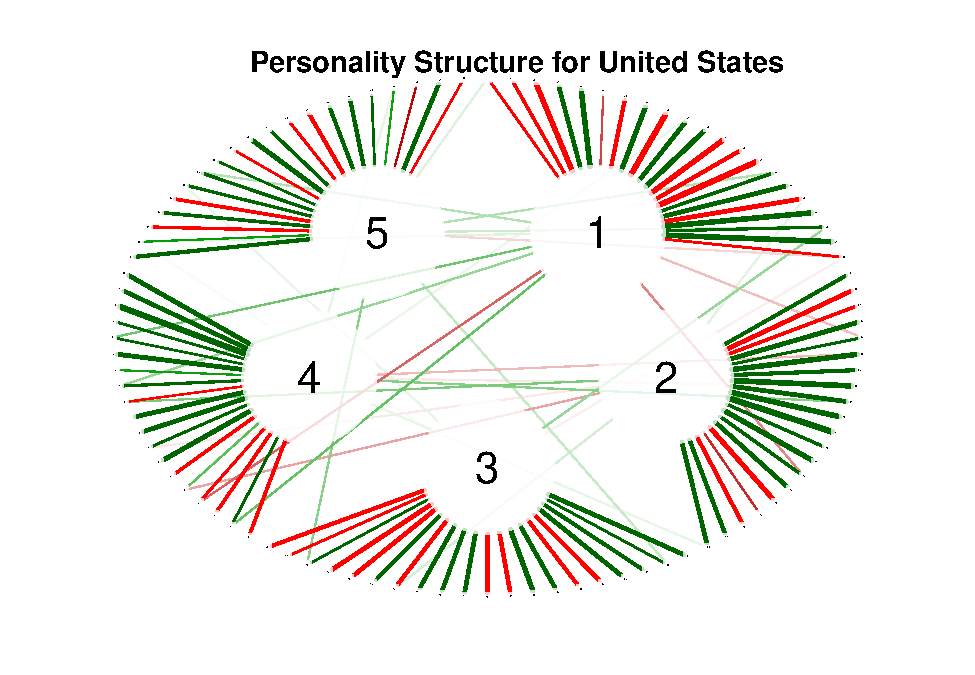
\includegraphics{final_manuscript_files/figure-latex/unnamed-chunk-3-1.pdf} 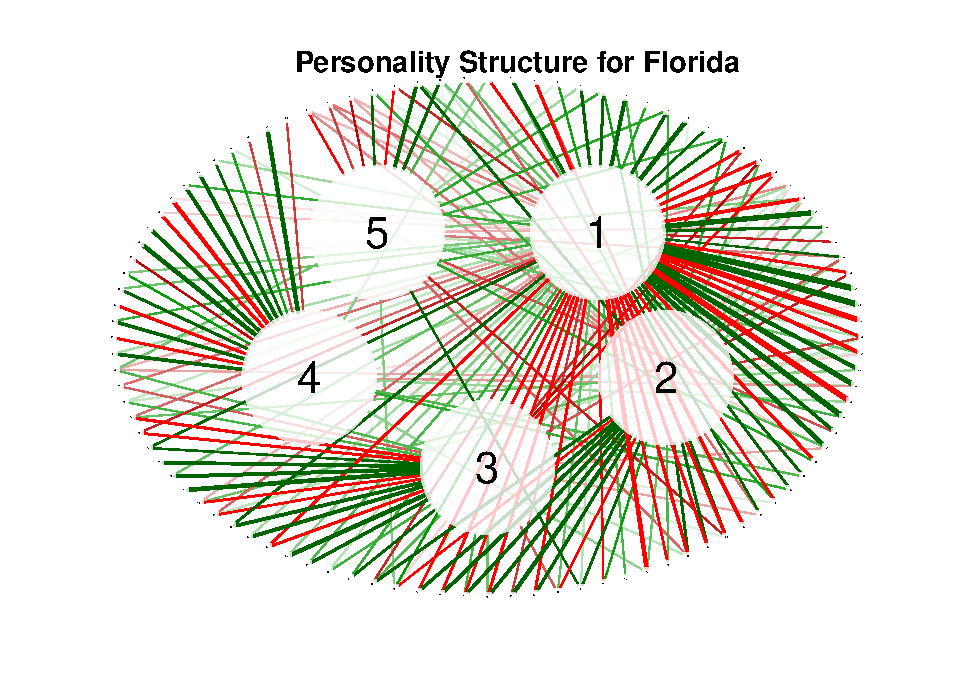
\includegraphics{final_manuscript_files/figure-latex/unnamed-chunk-3-2.pdf} 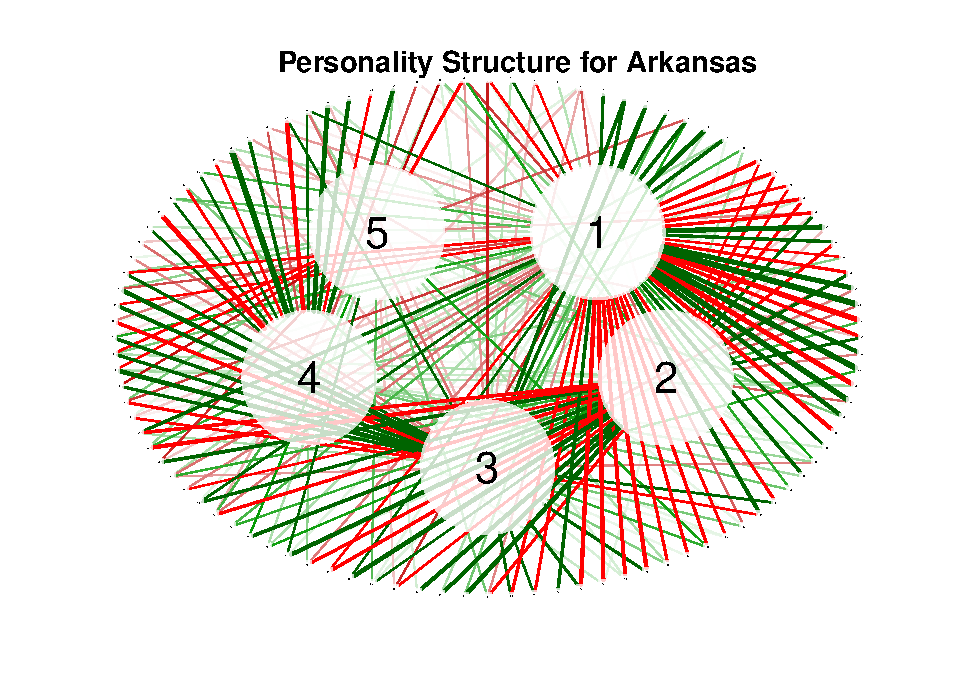
\includegraphics{final_manuscript_files/figure-latex/unnamed-chunk-3-3.pdf} 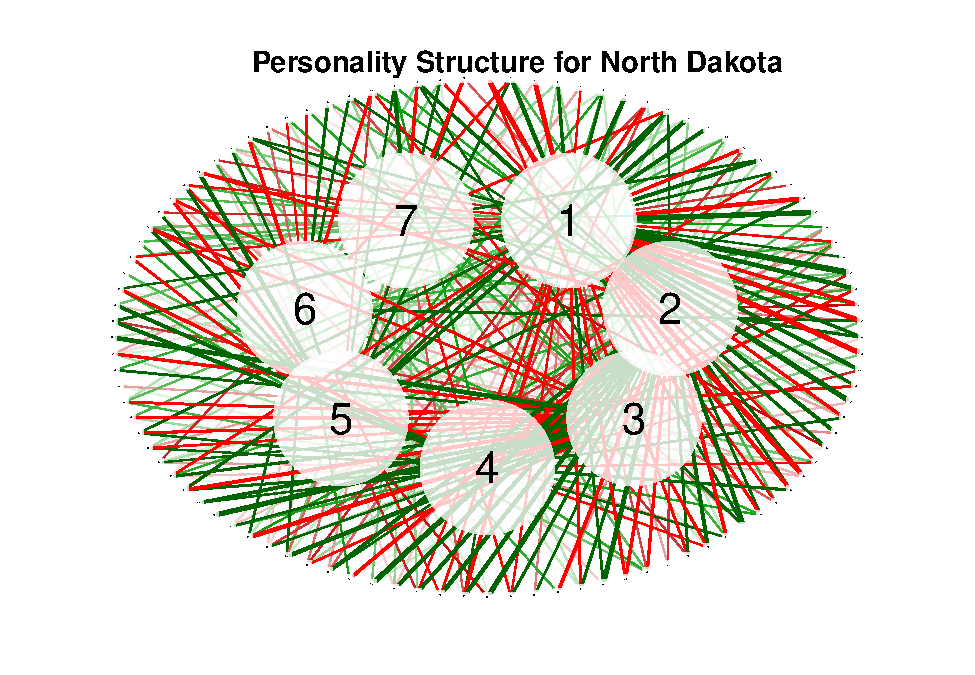
\includegraphics{final_manuscript_files/figure-latex/unnamed-chunk-3-4.pdf}

\hypertarget{discussion}{%
\section{Discussion}\label{discussion}}

\newpage

We used the following R packages for this manuscript: R {[}Version 4.1.1; R Core Team (2021){]} and the R-packages \emph{apaTables} {[}Version 2.0.8; Stanley (2021){]}, \emph{arsenal} {[}Version 3.6.3; Heinzen, Sinnwell, Atkinson, Gunderson, and Dougherty (2021){]}, \emph{dataverse} {[}Version 0.3.10; Kuriwaki, Beasley, and Leeper (2022){]}, \emph{dplyr} {[}Version 1.0.9; Wickham, François, Henry, and Müller (2022){]}, \emph{forcats} {[}Version 0.5.1; Wickham (2021){]}, \emph{ggplot2} {[}Version 3.3.6; Wickham (2016){]}, \emph{GPArotation} {[}Version 2022.4.1; Bernaards and I.Jennrich (2005){]}, \emph{here} {[}Version 1.0.1; Müller (2020){]}, \emph{kableExtra} {[}Version 1.3.4; Zhu (2021){]}, \emph{needs} {[}Version 0.0.3; Katz (2016){]}, \emph{papaja} {[}Version 0.1.0.9997; Aust and Barth (2020){]}, \emph{psych} {[}Version 2.2.5; Revelle (2022){]}, \emph{purrr} {[}Version 0.3.4; Henry and Wickham (2020){]}, \emph{qgraph} {[}Version 1.9.2; Epskamp, Cramer, Waldorp, Schmittmann, and Borsboom (2012){]}, \emph{readr} {[}Version 2.1.2; Wickham, Hester, and Bryan (2022){]}, \emph{rio} {[}Version 0.5.29; Chan, Chan, Leeper, and Becker (2021){]}, \emph{stringr} {[}Version 1.4.0; Wickham (2019){]}, \emph{tibble} {[}Version 3.1.7; Müller and Wickham (2022){]}, \emph{tidyr} {[}Version 1.2.0; Wickham and Girlich (2022){]}, and \emph{tidyverse} {[}Version 1.3.1; Wickham et al. (2019){]}

\newpage

\hypertarget{references}{%
\section{References}\label{references}}

\begingroup
\setlength{\parindent}{-0.5in}
\setlength{\leftskip}{0.5in}

\hypertarget{refs}{}
\begin{CSLReferences}{1}{0}
\leavevmode\vadjust pre{\hypertarget{ref-R-papaja}{}}%
Aust, F., \& Barth, M. (2020). \emph{{papaja}: {Create} {APA} manuscripts with {R Markdown}}. Retrieved from \url{https://github.com/crsh/papaja}

\leavevmode\vadjust pre{\hypertarget{ref-R-GPArotation}{}}%
Bernaards, C. A., \& I.Jennrich, R. (2005). Gradient projection algorithms and software for arbitrary rotation criteria in factor analysis. \emph{Educational and Psychological Measurement}, \emph{65}, 676--696.

\leavevmode\vadjust pre{\hypertarget{ref-R-rio}{}}%
Chan, C., Chan, G. C., Leeper, T. J., \& Becker, J. (2021). \emph{Rio: A swiss-army knife for data file i/o}.

\leavevmode\vadjust pre{\hypertarget{ref-condon2014international}{}}%
Condon, D. M., \& Revelle, W. (2014). The international cognitive ability resource: Development and initial validation of a public-domain measure. \emph{Intelligence}, \emph{43}, 52--64.

\leavevmode\vadjust pre{\hypertarget{ref-DVNux2f2IBBMG_2021}{}}%
Condon, D., Zabelina, D., \& Revelle, W. (2021). \emph{{Reproducibility Data for: Creative Achievement and Individual Differences}} (Version V3) {[}Data set{]}. Harvard Dataverse. \url{https://doi.org/10.7910/DVN/2IBBMG}

\leavevmode\vadjust pre{\hypertarget{ref-R-qgraph}{}}%
Epskamp, S., Cramer, A. O. J., Waldorp, L. J., Schmittmann, V. D., \& Borsboom, D. (2012). {qgraph}: Network visualizations of relationships in psychometric data. \emph{Journal of Statistical Software}, \emph{48}(4), 1--18.

\leavevmode\vadjust pre{\hypertarget{ref-R-arsenal}{}}%
Heinzen, E., Sinnwell, J., Atkinson, E., Gunderson, T., \& Dougherty, G. (2021). \emph{Arsenal: An arsenal of 'r' functions for large-scale statistical summaries}. Retrieved from \url{https://CRAN.R-project.org/package=arsenal}

\leavevmode\vadjust pre{\hypertarget{ref-R-purrr}{}}%
Henry, L., \& Wickham, H. (2020). \emph{Purrr: Functional programming tools}. Retrieved from \url{https://CRAN.R-project.org/package=purrr}

\leavevmode\vadjust pre{\hypertarget{ref-R-needs}{}}%
Katz, J. (2016). \emph{Needs: Attaches and installs packages}. Retrieved from \url{https://CRAN.R-project.org/package=needs}

\leavevmode\vadjust pre{\hypertarget{ref-R-dataverse}{}}%
Kuriwaki, S., Beasley, W., \& Leeper, T. J. (2022). \emph{Dataverse: R client for dataverse 4+ repositories}.

\leavevmode\vadjust pre{\hypertarget{ref-R-here}{}}%
Müller, K. (2020). \emph{Here: A simpler way to find your files}. Retrieved from \url{https://CRAN.R-project.org/package=here}

\leavevmode\vadjust pre{\hypertarget{ref-R-tibble}{}}%
Müller, K., \& Wickham, H. (2022). \emph{Tibble: Simple data frames}. Retrieved from \url{https://CRAN.R-project.org/package=tibble}

\leavevmode\vadjust pre{\hypertarget{ref-R-base}{}}%
R Core Team. (2021). \emph{R: A language and environment for statistical computing}. Vienna, Austria: R Foundation for Statistical Computing. Retrieved from \url{https://www.R-project.org/}

\leavevmode\vadjust pre{\hypertarget{ref-R-psych}{}}%
Revelle, W. (2022). \emph{Psych: Procedures for psychological, psychometric, and personality research}. Evanston, Illinois: Northwestern University. Retrieved from \url{https://CRAN.R-project.org/package=psych}

\leavevmode\vadjust pre{\hypertarget{ref-revelle2016web}{}}%
Revelle, W., Condon, D. M., Wilt, J., French, J. A., Brown, A., \& Elleman, L. G. (2016). Web and phone based data collection using planned missing designs. \emph{Sage Handbook of Online Research Methods (2nd Ed., P. 578-595). Sage Publications, Inc}.

\leavevmode\vadjust pre{\hypertarget{ref-R-apaTables}{}}%
Stanley, D. (2021). \emph{apaTables: Create american psychological association (APA) style tables}. Retrieved from \url{https://CRAN.R-project.org/package=apaTables}

\leavevmode\vadjust pre{\hypertarget{ref-R-ggplot2}{}}%
Wickham, H. (2016). \emph{ggplot2: Elegant graphics for data analysis}. Springer-Verlag New York. Retrieved from \url{https://ggplot2.tidyverse.org}

\leavevmode\vadjust pre{\hypertarget{ref-R-stringr}{}}%
Wickham, H. (2019). \emph{Stringr: Simple, consistent wrappers for common string operations}. Retrieved from \url{https://CRAN.R-project.org/package=stringr}

\leavevmode\vadjust pre{\hypertarget{ref-R-forcats}{}}%
Wickham, H. (2021). \emph{Forcats: Tools for working with categorical variables (factors)}. Retrieved from \url{https://CRAN.R-project.org/package=forcats}

\leavevmode\vadjust pre{\hypertarget{ref-R-tidyverse}{}}%
Wickham, H., Averick, M., Bryan, J., Chang, W., McGowan, L. D., François, R., \ldots{} Yutani, H. (2019). Welcome to the {tidyverse}. \emph{Journal of Open Source Software}, \emph{4}(43), 1686. \url{https://doi.org/10.21105/joss.01686}

\leavevmode\vadjust pre{\hypertarget{ref-R-dplyr}{}}%
Wickham, H., François, R., Henry, L., \& Müller, K. (2022). \emph{Dplyr: A grammar of data manipulation}. Retrieved from \url{https://CRAN.R-project.org/package=dplyr}

\leavevmode\vadjust pre{\hypertarget{ref-R-tidyr}{}}%
Wickham, H., \& Girlich, M. (2022). \emph{Tidyr: Tidy messy data}. Retrieved from \url{https://CRAN.R-project.org/package=tidyr}

\leavevmode\vadjust pre{\hypertarget{ref-R-readr}{}}%
Wickham, H., Hester, J., \& Bryan, J. (2022). \emph{Readr: Read rectangular text data}. Retrieved from \url{https://CRAN.R-project.org/package=readr}

\leavevmode\vadjust pre{\hypertarget{ref-wilt2011dynamic}{}}%
Wilt, J., Funkhouser, K., \& Revelle, W. (2011). The dynamic relationships of affective synchrony to perceptions of situations. \emph{Journal of Research in Personality}, \emph{45}(3), 309--321.

\leavevmode\vadjust pre{\hypertarget{ref-R-kableExtra}{}}%
Zhu, H. (2021). \emph{kableExtra: Construct complex table with 'kable' and pipe syntax}. Retrieved from \url{https://CRAN.R-project.org/package=kableExtra}

\end{CSLReferences}

\endgroup


\end{document}
